\chapter{System Design}
\label{cha:System Architecture}
This thesis work aims to implement a system that not only allows the least amount of data to be lost in case of power failure but also makes this management easy at the application level while hiding all the complexity of the system.\\
The communication stack is designed to reduce data loss issues during intermittent operation and make the best use of energy harvested from the surrounding environment.
\section{Architecture Diagram}
\label{sec:Architecture diagram}
The proposed system consists of four parts: \\
  \begin{figure}[H]
    \centerline{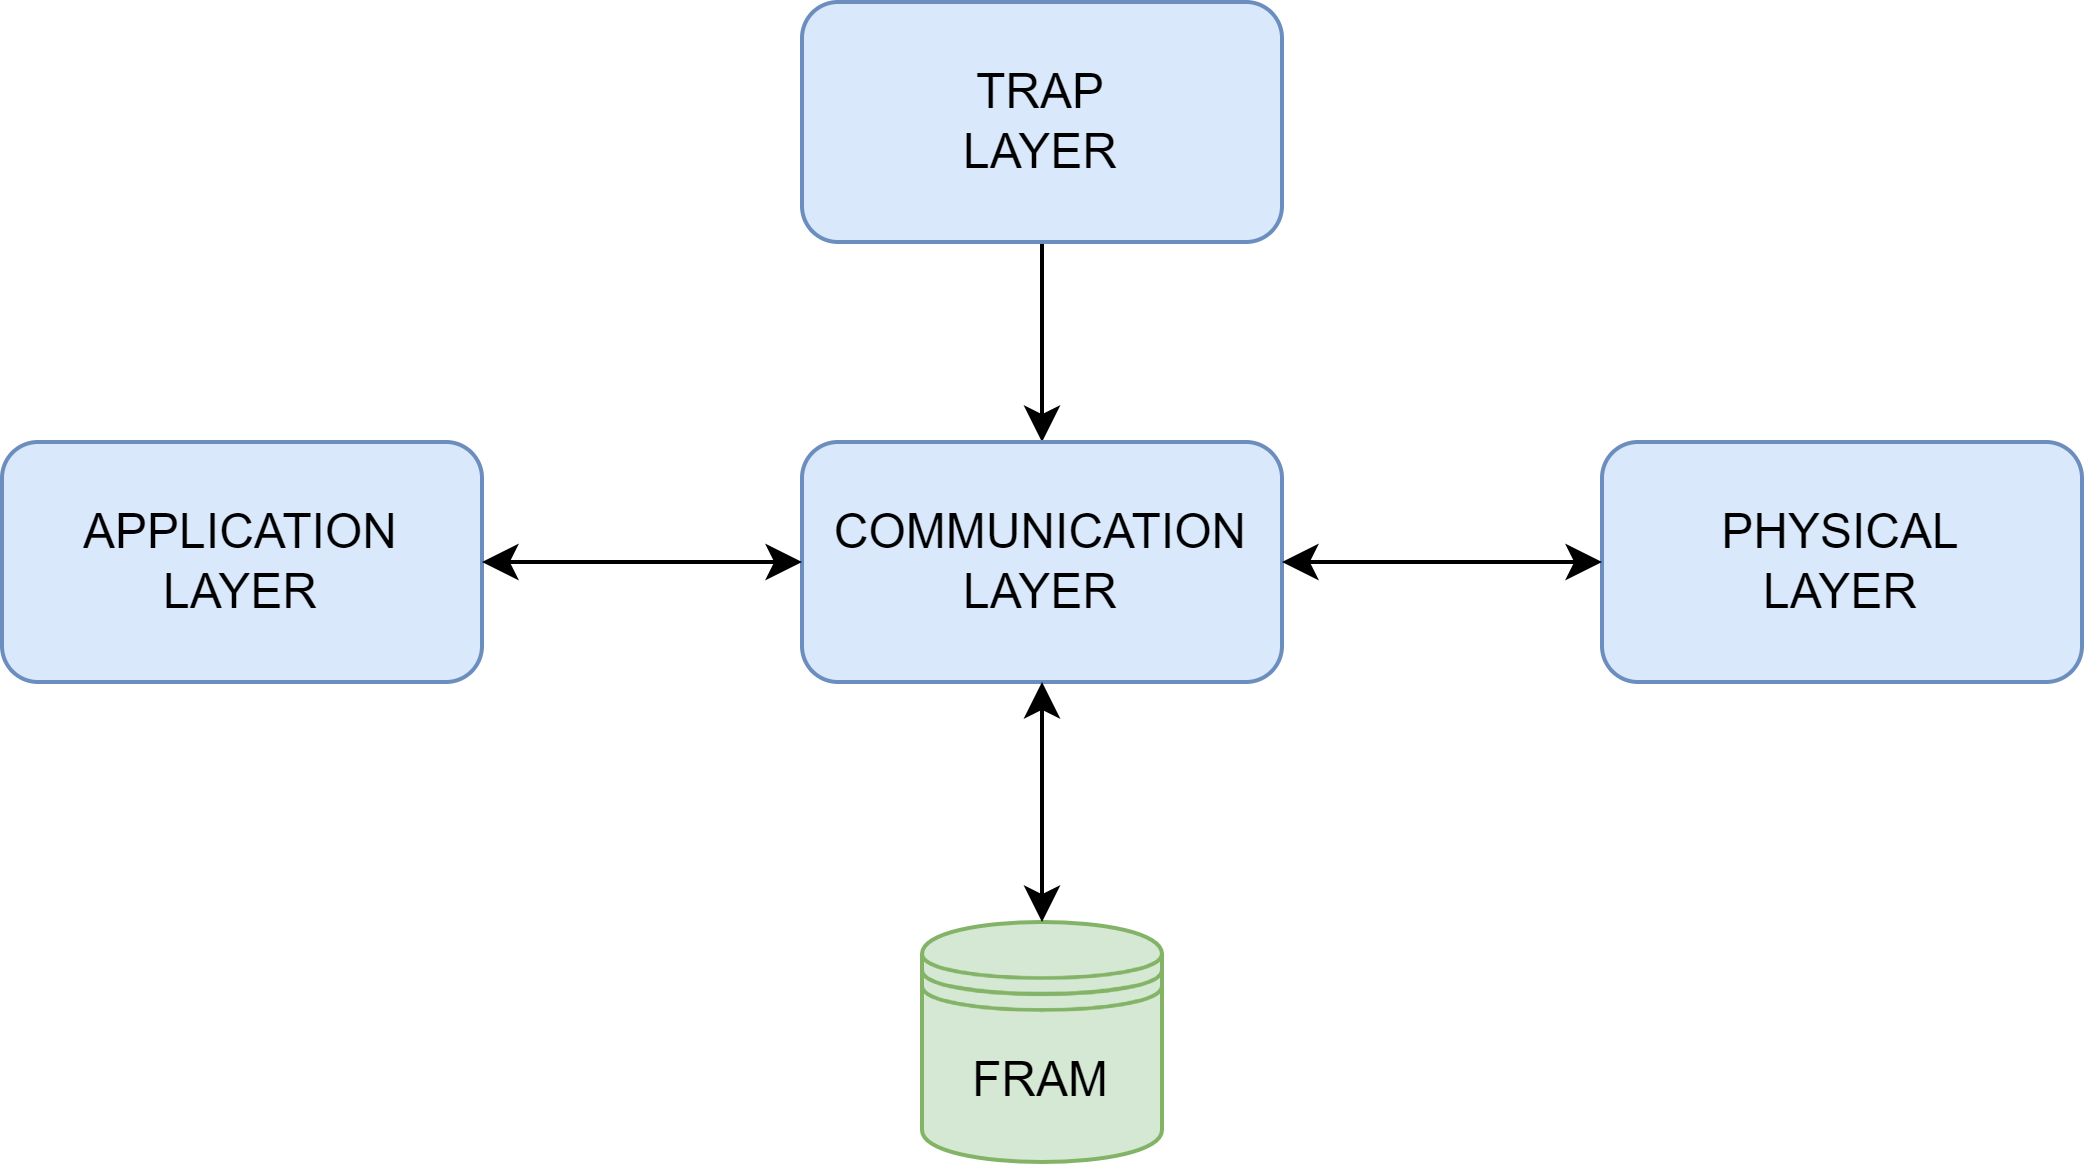
\psfig{file=Images/systemArchitecture.png,width=0.8\textwidth}}
    \caption{\footnotesize \centering System architecture diagram: Application Layer, TRAP Layer, Communication Layer and Physical Layer}
    \label{fig:SystemArchitectureDiagram}
  \end{figure}
 \subsection{Application Layer}
This section contains the abstractions that allow the programmer to develop an application using the implemented network stack.\\
The functions exposed by the Communication Layer allow high-level data sending and receiving. All memory management, transmitting, and receiving are executed automatically by the stack.\\
An example of an Application Layer, in pseudo code, might be as described below:\\
\begin{lstlisting}
....
while (1)
{
    value = collectDataFromSensor();
    destinationNode = 1;
    dataProduced(value, destinationNode);
    dataSend();
}
....
\end{lstlisting}
\subsection{TRAP Layer}
The Trap Layer is the layer that implements the TRAP protocol.\\
It is based on the use of timers for repetitive burst sending, OOK modulation, and sending node identification.\\
The bursts contain encoding of the energy level of the sending node. Each neighboring node in the network sends its energy level at fixed intervals.\\
Recognition of the sending node is accomplished by an analysis of the burst sending frequency.\\
\subsection{Communication Layer}
Communication Layer is the part of the system responsible for sending and receiving data from the Physical Layer and the Application Layer.\\
The Communication Layer does much more than what has just been explained: it is responsible for managing the data within non-volatile memory (FRAM \cite{FRAM})  so it is the heart of the system.\\
FRAM management consists of saving and retrieving data; this mechanism helps limit packet losses during power failures.\\
\subsection{Physical Layer}
The Physical Layer is the layer responsible for actually sending and receiving packets.\\
It is easily replaceable and allows the use of different transmission technologies such as backscatter communication or visible-light communication.\\
In this implementation, the choice fell on the use of a UART communication.\\
A whole chapter will not be devoted to explaining the layer as it is of little significance to the implementation. It will be mentioned in the evaluation section to give context to the tests performed.
  
\newpage




